\rokegz{$date$ r.}
\rokak{2018/2019}
\semestr{Zima}
\stopien{II}
\kierunek{Informatyka}
\instytut{informatyki}
\jednostka{Instytut Informatyki}
\specjalnosc{Inżynieria Systemów Informatycznych}
\typ{magisterska}
\autor{$author$}
\nralbumu{1}
\adresa{1007 Mountain Drive}
\adresb{Gotham City}
\foto{portrait.jpeg}
\dataurodzenia{February 2nd, 1974}
\datarozpoczecia{October 1st, 2010}

\opiekun{Lucius Fox PhD}

\tytul{$tytul$}
\tytulen{An automated system of crime evaluation}

\zyciorys{Bruce Wayne podróżuje od 14. roku życia. Ukończył kursy na Sorbonie i innych uniwersytetach europejskich. Nigdy nie pozostał na uczelni na tyle długo by ukończyć semestr, stąd w naukach czy inżynierii nie legitymuje się żadnym tytułem - niemal na pewno zna jednak osobiście ministra edukacji urzędującego w kraju czytelnika. Poza życiem akademickim przyswoił rozmaite sztuki walki w czasie swych licznych podróży oraz opracował szerokie portfolio wynalazków. Spośród tych ostatnich większość pozostaje ściśle tajna jako prywatny majątek rodzinnej korporacji.\\[3mm]
Poniżej podpis:}

\streszczenie{$streszczenie$}

\streszczenieen{The aim of this thesis is design and publication of a prototype of a solution to the problem of remote aquisition of information about patterns emergin in data classified as sensitive by law.\\[3mm]
The mentioned aim is motivated by a vision of lessening the attack surface where data of personal nature is concerned; also - of limiting the cost of additional infrastructure needed by the provider in order to implement the service. The proposed model achieves that through engagement of the user, who in turn gains additional possibilities. In this document an architecture is presented, designed to fulfill a specific purpose of automatizing certification of flexible users of electric energy.\\[3mm]
Used for the purpose of achieving the stated goal were original, customly designed algorithms based on patterns of asynchronous and parallel programming, together with their prototypical implementations.}

\slowakluczowe{$keywords$}
\slowakluczoween{DSR, flexibility estimation, architecture, asynchronous programming.}

$if(draft)$
\clearpage
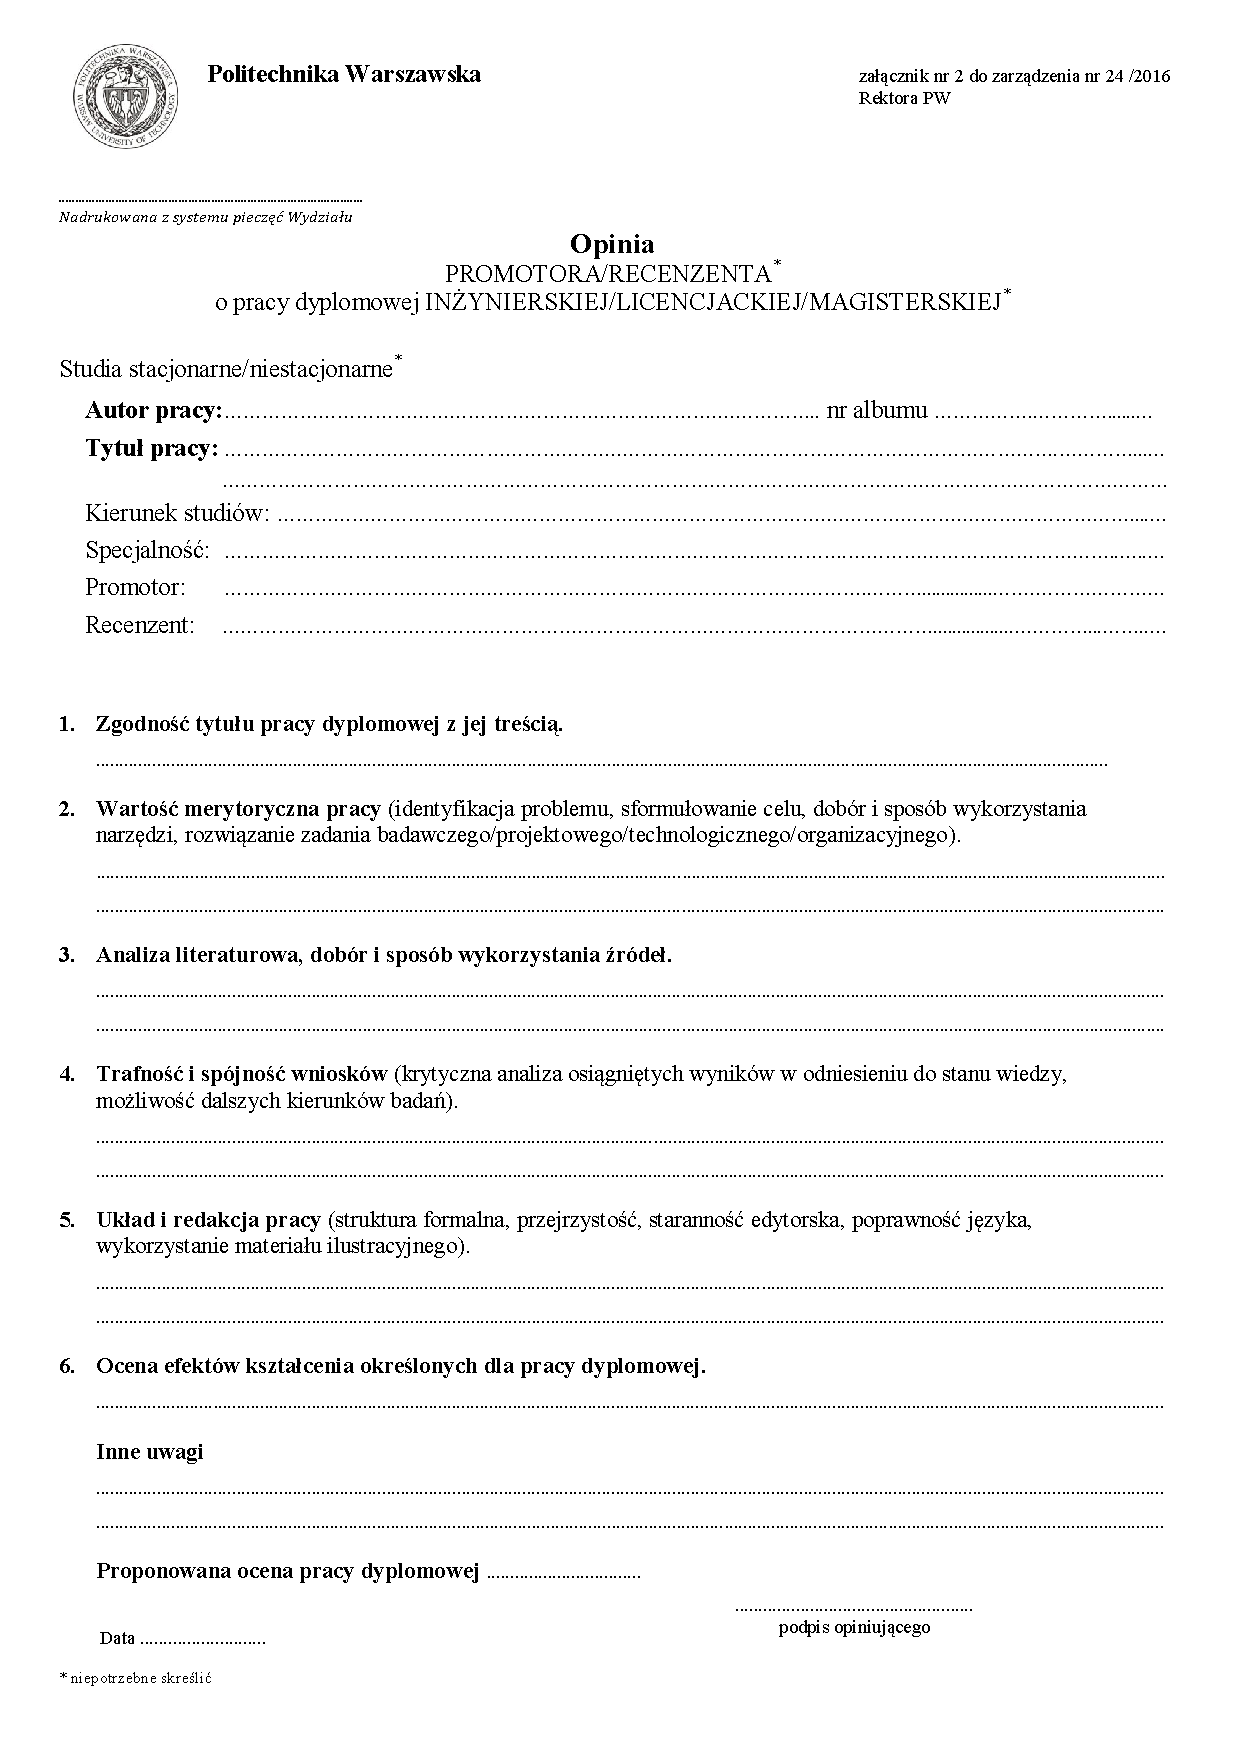
\includepdf[pages=-]{test/recenzja-nowy-formularz.pdf}
\section*{Najnowsze zmiany w projekcie}
\thispagestyle{empty}
$endif$

$if(customtitlepage)$
\maketitle
$endif$

$if(infocard)$
\makeinfo
$endif$

$if(abstracts)$
\makeabstracts
$endif$

\thispagestyle{empty}
\cleartooddpage
\tableofcontents

\cleartooddpage
